\chapter{Catene di Markov}
\label{cap:catene-markov}

\scan{72}
Gli algoritmi randomizzati visti finora ci hanno portati più volte a studiare una
passeggiata aleatoria: la visita casuale di un grafo, di cui abbiamo stimato il
\emph{cover time}, e l'algoritmo per \textsc{2-cnf-sat}, che è un random walk sulla
retta $\{0,1,\dots,n\}$. La nozione generale di cui tutti questi processi sono casi
particolari è quella di \emph{catena di Markov}, alla quale è dedicato questo
capitolo. Il riferimento bibliografico classico è W.~Feller, \emph{An Introduction to
Probability Theory and Its Applications}, Vol.~I, cap.~XV; per il taglio algoritmico,
Motwani--Raghavan, \emph{Randomized Algorithms}, cap.~6.


\section{Definizione}

\scan{73}
Feller le introduce a partire da una successione di prove ripetute, e ne descrive la
probabilità di un'\emph{intera} sequenza di esiti.

\begin{definizione}[Catena di Markov, nella forma di Feller]\label{def:mc-feller}
  Si consideri una successione di prove (\emph{trials}, esperimenti) i cui esiti
  possibili sono $E_1, E_2, \dots$\,; le prove formano una \emph{catena di Markov} se la
  probabilità che gli esiti si verifichino, nell'ordine, $E_{j_0}, E_{j_1}, \dots,
  E_{j_t}$ si fattorizza come
  \[
    \Pr\bigl\{(E_{j_0}, E_{j_1}, \dots, E_{j_t})\bigr\}
      \;=\; a_{j_0} \cdot P_{j_0 j_1} \cdot P_{j_1 j_2} \cdot P_{j_2 j_3}
            \cdots P_{j_{t-1} j_t},
  \]
  dove
  \begin{itemize}
    \item $a_{j_0}$ è la probabilità che si verifichi $E_{j_0}$, cioè la distribuzione
          iniziale sugli esiti;
    \item $P_{j_{k-1} j_k}$ è la probabilità che si verifichi $E_{j_k}$ \emph{a
          condizione che} si sia verificato $E_{j_{k-1}}$.
  \end{itemize}
\end{definizione}

\paragraph{Memoryless (property).}
Tutto il contenuto della definizione sta nella forma dei fattori: la probabilità del
$k$-esimo esito è condizionata al solo esito immediatamente precedente, non all'intera
storia della successione. Oltre al presente, il passato non porta informazione.

D'ora in avanti chiameremo \emph{stati} gli esiti possibili e denoteremo con $S$
l'insieme che li raccoglie.

\subsection{Catene di Markov discrete}

\scan{75}
L'aggettivo \emph{discreta} si riferisce agli stati: sono «ben distinti», cioè $S$ è un
insieme (per noi \emph{finito}) di stati. In questa forma la definizione si dà
direttamente sulle variabili aleatorie.

\begin{definizione}[Catena di Markov discreta]\label{def:catena-markov}
  Una \emph{catena di Markov} su $S$ è un \emph{processo stocastico} su $S$, cioè una
  successione di variabili aleatorie
  \[
    X_0,\; X_1,\; \dots,\; X_t,\; X_{t+1},\; \dots
  \]
  a valori in $S$, che soddisfa la \emph{proprietà di Markov}: per ogni $t \ge 0$ e per
  ogni scelta di stati $i_0, \dots, i_t, j \in S$
  \[
    \Pr\bigl[X_{t+1} = j \;\big|\; X_0 = i_0,\, \dots,\, X_t = i_t\bigr]
    \;=\;
    \Pr\bigl[X_{t+1} = j \;\big|\; X_t = i_t\bigr].
  \]
\end{definizione}

\begin{osservazione}
  Le due definizioni dicono la stessa cosa. Sviluppando il condizionamento un passo
  alla volta, la proprietà di Markov dà infatti
  \[
    \Pr\bigl[X_0 = i_0,\, X_1 = i_1,\, \dots,\, X_t = i_t\bigr]
    \;=\; a_{i_0}\, P_{i_0 i_1} P_{i_1 i_2} \cdots P_{i_{t-1} i_t},
  \]
  che è esattamente la fattorizzazione della Definizione~\ref{def:mc-feller}, purché i fattori
  $P_{ij}$ non dipendano dall'istante $t$ in cui la transizione avviene: è l'ipotesi di
  \emph{omogeneità nel tempo}, implicita nella scrittura di Feller e assunta d'ora in
  poi. È proprio l'omogeneità che consente di raccogliere tutte le probabilità di
  transizione in un'unica matrice.
\end{osservazione}

\scan{73}
Tutta l'informazione sul passato che serve a predire il futuro è dunque contenuta nello
stato corrente:

\begin{center}
  \emph{Condizionatamente al presente, il futuro non dipende dal passato.}
\end{center}

\subsection{Due domande sulla proprietà di Markov}

\scan{74}
Lo slogan va però maneggiato con cura. Siano $X_0, X_1, X_2, \dots$ una catena di
Markov e siano $A$ e $B$ due sottoinsiemi di stati.

\begin{domanda}
\begin{enumerate}
  \item È vero che
  \[
    \Pr\bigl\{\, X_2 \in B \;\big|\; X_1 = x_1 \,\wedge\, X_0 \in A \,\bigr\}
    \;=\;
    \Pr\bigl\{\, X_2 \in B \;\big|\; X_1 = x_1 \,\bigr\}\;?
  \]
  \item È vero che
  \[
    \Pr\bigl\{\, X_2 \in B \;\big|\; X_1 \in A \,\wedge\, X_0 = x_0 \,\bigr\}
    \;=\;
    \Pr\bigl\{\, X_2 \in B \;\big|\; X_1 \in A \,\bigr\}\;?
  \]
\end{enumerate}
\end{domanda}

La prima uguaglianza è vera; la seconda, in generale, no.

\begin{osservazione}
Nella (1) il condizionamento fissa \emph{esattamente} lo stato presente
($X_1 = x_1$): per la proprietà di Markov l'informazione aggiuntiva sul passato
($X_0 \in A$) è irrilevante e l'uguaglianza vale.

Nella (2), invece, l'evento $X_1 \in A$ non individua un singolo stato presente.
Condizionando e poi decomponendo su quale stato di $A$ sia stato effettivamente
raggiunto,
\begin{align*}
  &\Pr\bigl\{X_2 \in B \mid X_1 \in A \wedge X_0 = x_0\bigr\} \\[2pt]
  &\qquad\qquad =\;
  \sum_{a \in A}
    \Pr\bigl\{X_1 = a \mid X_1 \in A \wedge X_0 = x_0\bigr\}\;
    \Pr\bigl\{X_2 \in B \mid X_1 = a\bigr\},
\end{align*}
si vede che sapere $X_0 = x_0$ cambia i \emph{pesi} con cui gli stati di $A$
entrano nella media (basta che da $x_0$ qualche stato di $A$ sia irraggiungibile
perché i pesi cambino): il passato torna a contare e l'uguaglianza cade. La
proprietà di Markov si applica al presente \emph{puntuale}, non al presente
«sfocato» in un insieme di stati.
\end{osservazione}

\begin{dubbio}
A margine della (2) il quaderno annota: «sì, nel caso in cui la probabilità di
passare da $x_0$ a qualche stato di $A$ è $0$» (la prima parola, sottolineata, si
legge «sì», ma potrebbe essere «se»). Le due letture di «qualche stato di $A$»
portano in direzioni opposte, e la nota non basta a decidere fra loro. Se la si
intende come $\Pr\{X_1 \in A \mid X_0 = x_0\} = 0$, allora l'evento condizionante
$\{X_1 \in A \wedge X_0 = x_0\}$ è impossibile e la (2) non è né vera né falsa:
il membro sinistro non è nemmeno definito. Se invece «qualche stato» va inteso
come «un particolare stato di $A$», la nota descrive proprio il meccanismo per cui
la (2) \emph{fallisce}, quello dell'osservazione qui sopra: se da $x_0$ un certo
$a \in A$ non è raggiungibile, i pesi con cui gli stati di $A$ entrano nella media
cambiano.
\end{dubbio}


\section{Matrice di transizione e vettore di stato}

\scan{73}
Supponiamo d'ora in avanti che gli stati siano in numero finito, $S = \{1, \dots, n\}$
(identifichiamo cioè l'esito $E_i$ con lo stato $i$), e raccogliamo le probabilità di
transizione nella \emph{matrice di transizione}
\[
  P \;=\;
  \begin{pmatrix}
    P_{11} & \cdots & P_{1n} \\
    \vdots &        & \vdots \\
    P_{n1} & \cdots & P_{nn}
  \end{pmatrix}.
\]
Ogni \emph{riga} di $P$ è una distribuzione di probabilità sugli $n$ stati — la riga
$i$-esima dice dove si può andare a partire da $i$, e con quale probabilità — sicché
\[
  \sum_{j=1}^{n} P_{ij} \;=\; 1 \qquad \text{per ogni } i = 1, \dots, n .
\]
Una matrice quadrata a entrate non negative con questa proprietà si dice
\emph{stocastica}.

\begin{osservazione}
  Il quaderno affianca a questa anche l'identità per colonne $\sum_{i=1}^{n} P_{ij} = 1$.
  Non è però una richiesta della definizione: vale soltanto per le matrici
  \emph{doppiamente stocastiche}, che sono un caso particolare. Lo è, per esempio, la
  passeggiata aleatoria simmetrica sul ciclo della Sezione~\ref{sec:mc-esempio-ciclo}, ed è
  esattamente il motivo per cui in quel caso la distribuzione limite risulta uniforme.
\end{osservazione}

\paragraph{Notazione.}
\scan{75}
\begin{itemize}
  \item $P_{ij}$ è la probabilità di transizione da $i$ a $j$ in \emph{un} passo,
        \[
          P_{ij} \;=\; \Pr[X_{t+1} = j \mid X_t = i],
        \]
        e per l'ipotesi di omogeneità non dipende da $t$;
  \item $P^{(t)}_{ij}$ è la probabilità di andare da $i$ a $j$ in \emph{esattamente}
        $t$ passi,
        \[
          P^{(t)}_{ij} \;=\; \Pr[X_t = j \mid X_0 = i].
        \]
\end{itemize}

\paragraph{Stato iniziale.} Per $X_0$ ci sono due possibilità: o è \emph{fisso},
oppure viene \emph{generato da una distribuzione} iniziale sugli stati.

\medskip

\scan{73}
Alla matrice $P$ si associa naturalmente un grafo orientato sull'insieme $S$ degli
stati: i nodi sono gli stati e c'è un arco da $i$ a $j$ quando $P_{ij} > 0$. È il punto
di vista che useremo sistematicamente più avanti.

\begin{figure}[H]
  \centering
  % p73-spazio-stati -- lo spazio degli stati S come "patata" con dentro un
% pezzo del grafo di transizione (quaderno, pag. 73).
% Tre stati s1, s2, s3; arco s1->s2, coppia s1<->s3 (lente), cappio su s3.
\begin{tikzpicture}[
    font=\footnotesize,
    stato/.style={circle,draw,line width=0.7pt,fill=white,
                  inner sep=0pt,minimum size=5.5pt},
    arco/.style={line width=0.7pt,-{Stealth[length=4.5pt,width=3.5pt]}}]

  %% ------------------- la "patata": l'insieme S degli stati -------------
  \draw[line width=0.8pt,gray]
    plot[smooth cycle,tension=0.75]
    coordinates {(0.30,1.80) (1.10,3.00) (2.40,3.35) (3.10,2.70)
                 (3.90,3.30) (5.00,3.10) (5.70,2.00) (5.20,0.90)
                 (4.20,0.25) (3.10,0.55) (2.40,0.15) (1.20,0.50)
                 (0.45,1.10)};

  %% ------------------- glossa esterna ----------------------------------
  \node[anchor=east,align=center] (etS) at (-0.70,2.15) {$S$\\[1pt]stati};
  \draw[line width=0.5pt,gray] (etS.east) -- (0.34,1.90);

  %% ------------------- gli stati ---------------------------------------
  \node[stato] (s1) at (1.80,1.30) {};
  \node[stato] (s2) at (2.65,2.25) {};
  \node[stato] (s3) at (3.95,1.55) {};

  \node[anchor=east]       at ([xshift=-2pt]s1.west)              {$s_1$};
  \node[anchor=south]      at ([yshift=2pt]s2.north)              {$s_2$};
  \node[anchor=north west] at ([shift={(1pt,-2pt)}]s3.south east) {$s_3$};

  %% ------------------- transizioni --------------------------------------
  \draw[arco] (s1) to[bend left=32] (s2);          % s1 -> s2
  \draw[arco] (s1) to[bend left=24] (s3);          % s1 -> s3
  \draw[arco] (s3) to[bend left=24] (s1);          % s3 -> s1
  \draw[arco] (s3) to[out=62,in=2,looseness=1,min distance=7mm] (s3); % cappio

\end{tikzpicture}

  \caption{L'insieme $S$ degli stati e alcune transizioni possibili fra di essi.}
  \label{fig:p73-spazio-stati}
\end{figure}

Letta così, una catena di Markov è \emph{una generalizzazione della nozione di
funzione}: a ogni stato non è associato un unico successore, ma una distribuzione di
probabilità sui successori possibili. Il caso deterministico si riottiene quando ogni
riga di $P$ contiene un solo $1$ e tutti gli altri elementi nulli.
L'osservazione è attribuita, nel quaderno, a \dubbioinl{J.~T.~Schwartz}.

\scan{75}
Quando gli stati sono pochi, il grafo di transizione si disegna per esteso, con le
probabilità come etichette degli archi.

\begin{figure}[H]
  \centering
  % p75-mc-due-stati -- diagramma di transizione di una catena a due stati
% (schizzo a matita nel margine, quaderno pag. 75).
% Le etichette sono quelle del quaderno: le uscite da 2 non sommano a 1,
% l'incongruenza e' discussa nell'ambiente "dubbio" subito dopo la figura.
\begin{tikzpicture}[
    font=\footnotesize,
    stato/.style={circle,draw,line width=0.7pt,fill=white,
                  inner sep=1pt,minimum size=7mm},
    arco/.style={line width=0.7pt,-{Stealth[length=5pt,width=4pt]}}]

  \node[stato] (u) at (0,0)   {$1$};
  \node[stato] (v) at (3.5,0) {$2$};

  % 1 -> 2 : arco che scavalca i due nodi
  \draw[arco] (u) to[bend left=45]  node[above,pos=0.5]{$0{,}8$} (v);
  % 2 -> 1 : arco di ritorno, sotto
  \draw[arco] (v) to[bend left=45]  node[below,pos=0.72]{$0{,}2$} (u);

  % cappi
  \draw[arco] (u) to[out=155,in=205,looseness=1,min distance=12mm]
              node[above left,pos=0.5,inner sep=1.5pt]{$0{,}2$} (u);
  \draw[arco] (v) to[out=-25,in=25,looseness=1,min distance=12mm]
              node[below right,pos=0.5,inner sep=1.5pt]{$0{,}2$} (v);

\end{tikzpicture}

  \caption{Catena di Markov a due stati, abbozzata a margine della pagina.}
  \label{fig:p75-mc-due-stati}
\end{figure}

\begin{dubbio}
  Nello schizzo le probabilità uscenti dallo stato $2$ sommano a $0{,}4$ e non a $1$:
  una delle due etichette $0{,}2$ che lo riguardano (il cappio su $2$ oppure l'arco di
  ritorno $2 \to 1$) dovrebbe valere $0{,}8$, ma dal quaderno non si capisce quale
  delle due.
\end{dubbio}

\medskip

Della catena interessa infine, a ogni istante, non tanto il singolo stato occupato
quanto la distribuzione di probabilità sugli stati.

\begin{definizione}[Vettore di stato, \emph{state probability vector}]\label{def:state-probability-vector}
  \scan{77}
  Il \emph{vettore di probabilità di stato} al tempo $t$ è il vettore riga
  \[
    \vec{q}^{\,(t)} \;=\; \bigl(q^{(t)}_{1},\, \dots,\, q^{(t)}_{n}\bigr),
  \]
  dove $q^{(t)}_{i}$ è la probabilità che la catena si trovi nello stato $i$ al tempo $t$.
\end{definizione}

Il vettore $\vec{q}^{\,(t)}$ è dunque la distribuzione dello stato al tempo $t$:
rappresenta la distribuzione della probabilità di visita di un random walk sul grafo di
transizione. Il passo della catena si ottiene moltiplicando il vettore (riga) di stato
per la matrice di transizione:
\[
  \vec{q}^{\,(t+1)} \;=\; \vec{q}^{\,(t)} \times P ,
  \qquad\text{e quindi}\qquad
  \vec{q}^{\,(t)} \;=\; \vec{q}^{\,(0)}\, P^{t} .
\]


\section{Un esempio: la passeggiata aleatoria sul ciclo}
\label{sec:mc-esempio-ciclo}

\scan{74}

\begin{esempio}\label{es:ciclo6}
Passeggiata aleatoria pigra sul ciclo a sei stati $\{0,1,2,3,4,5\}$: da ogni
stato ci si sposta al vicino precedente, si resta fermi, oppure ci si sposta al
vicino successivo, ciascuna cosa con probabilità $1/3$.

\begin{figure}[H]
\centering
% p74-ciclo6 -- passeggiata aleatoria "pigra" sul ciclo a sei stati
% (quaderno, pag. 74).  Sei stati 0..5 disposti in cerchio in senso orario
% a partire dall'alto; ogni stato ha un cappio e due archi (uno per verso)
% verso ciascun vicino.  Tutte le transizioni hanno probabilita' 1/3.
\begin{tikzpicture}[
    font=\footnotesize,
    stato/.style={circle,draw,line width=0.7pt,fill=white,
                  inner sep=1pt,minimum size=7mm},
    arco/.style={line width=0.7pt,-{Stealth[length=4.5pt,width=3.5pt]}}]

  %% ------------------- i sei stati --------------------------------------
  \foreach \n/\ang in {0/90, 1/30, 2/-30, 3/-90, 4/210, 5/150}
    \node[stato] (s\n) at (\ang:2.2) {$\n$};

  %% ------------------- archi fra vicini (uno per verso) -----------------
  \foreach \i/\j in {0/1, 1/2, 2/3, 3/4, 4/5, 5/0} {
    \draw[arco] (s\i) to[bend left=16] (s\j);
    \draw[arco] (s\j) to[bend left=16] (s\i);
  }

  %% ------------------- cappi, radiali verso l'esterno -------------------
  \foreach \n/\uscita/\entrata in {0/112/68, 1/52/8, 2/-8/-52,
                                   3/-68/-112, 4/232/188, 5/172/128}
    \draw[arco] (s\n) to[out=\uscita,in=\entrata,looseness=1,min distance=8mm]
                (s\n);

  %% ------------------- glossa al centro ---------------------------------
  \node[align=center] at (0,0) {ogni arco:\\[1pt]$\tfrac13$};

\end{tikzpicture}

\caption{La catena dell'esempio: sei stati disposti in cerchio, ciascuno con un
cappio e due archi (uno per verso) verso i due vicini; ogni arco ha probabilità
$1/3$.}
\label{fig:p74-ciclo6}
\end{figure}

Partendo da $i$, qual è la probabilità del passaggio $i \to j$?
\[
  P_{ij} \;=\;
  \begin{cases}
    \tfrac13 & j = i-1 \quad(\text{un passo indietro}),\\[2pt]
    \tfrac13 & j = i \phantom{{}-1} \quad(\text{fermo}),\\[2pt]
    \tfrac13 & j = i+1 \quad(\text{un passo avanti}),\\[2pt]
    0        & \text{altrimenti,}
  \end{cases}
\]
dove gli indici sono intesi modulo $6$.

Facendo partire la catena dallo stato $2$, il vettore di stato evolve così:
\begin{align*}
  \vec{q}^{\,(0)} &= \bigl(0,\;0,\;1,\;0,\;0,\;0\bigr), \\
  \vec{q}^{\,(1)} &= \bigl(0,\;\tfrac13,\;\tfrac13,\;\tfrac13,\;0,\;0\bigr)
               && \text{in $1$ passo,}\\
  \vec{q}^{\,(2)} &= \bigl(\tfrac19,\;\tfrac29,\;\tfrac13,\;\tfrac29,\;\tfrac19,\;0\bigr)
               && \text{in $2$ passi,}\\
  &\;\;\;\vdots \\
  \vec{q}^{\,(t)} &\;\xrightarrow[\;t\to\infty\;]{}\;
               \bigl(\tfrac16,\;\tfrac16,\;\tfrac16,\;\tfrac16,\;\tfrac16,\;\tfrac16\bigr).
\end{align*}
\end{esempio}

\begin{osservazione}
La matrice $P$ di questa catena è doppiamente stocastica (ogni riga e ogni colonna
somma a $1$); la catena è inoltre irriducibile, perché il ciclo è connesso, e
aperiodica, perché i cappi danno periodo $1$. Nel linguaggio della
Sezione~\ref{sec:mc-stazionaria} si tratta dunque di una catena ergodica: il
Teorema~\ref{thm:mc-fondamentale} ne garantisce la distribuzione stazionaria, e per le
catene ergodiche finite la distribuzione al tempo $t$ vi converge qualunque sia lo stato
di partenza --- è il limite scritto sopra. Che tale limite sia la distribuzione uniforme
lo dice la doppia stocasticità: se ogni colonna di $P$ somma a $1$, il vettore costante
$\vec{\pi} = \bigl(\tfrac16,\dots,\tfrac16\bigr)$ soddisfa $\vec{\pi} = \vec{\pi}P$.
\end{osservazione}

\begin{osservazione}
Il passo elementare $\vec{q}^{\,(t+1)} = \vec{q}^{\,(t)}P$ è, per questa catena, una
\emph{convoluzione}: per ogni stato $j$
\[
  q^{(t+1)}_{j} \;=\;
  \tfrac13\Bigl(q^{(t)}_{j-1} + q^{(t)}_{j} + q^{(t)}_{j+1}\Bigr),
\]
cioè si fa scorrere sulla distribuzione corrente la finestra di pesi
$\bigl(\tfrac13,\tfrac13,\tfrac13\bigr)$ e si sommano i tre contributi.

\begin{figure}[H]
\centering
% p74-convoluzione -- il passo q^(t+1) = q^(t) P della passeggiata sul ciclo
% letto come convoluzione (quaderno, pag. 74, schizzo a matita).
% Sopra: i tre valori adiacenti della distribuzione corrente, pesati 1/3 e
% sommati nel valore nuovo.  Sotto: la finestra (1/3,1/3,1/3) che scorre.
\begin{tikzpicture}[
    font=\footnotesize,
    linea/.style={line width=0.7pt},
    freccia/.style={line width=0.7pt,-{Stealth[length=4.5pt,width=3.5pt]}}]

  %% ---------- le tre posizioni adiacenti della distribuzione al tempo t --
  \foreach \i/\et in {0/{q^{(t)}_{j-1}}, 1/{q^{(t)}_{j}}, 2/{q^{(t)}_{j+1}}} {
    \node at ({1.7*\i},2.55) {$\et$};
    \draw[linea] ({1.7*\i},2.25) -- ({1.7*\i},1.95);   % trattino verticale
    \node at ({1.7*\i},1.72) {$\tfrac13$};             % peso
  }
  \node at (0.85,1.72) {$+$};
  \node at (2.55,1.72) {$+$};

  %% ---------- la graffa che raccoglie i tre contributi -------------------
  \draw[linea,decorate,decoration={brace,amplitude=5pt,mirror,raise=1pt}]
        (-0.55,1.40) -- (3.95,1.40);
  \draw[freccia] (1.7,1.02) -- (1.7,0.62);
  \node at (1.7,0.38) {$q^{(t+1)}_{j}$};

  %% ---------- la finestra di convoluzione --------------------------------
  \draw[linea] (-0.85,-1.20) rectangle (4.25,-0.50);
  \draw[linea] (0.85,-1.20) -- (0.85,-0.50);
  \draw[linea] (2.55,-1.20) -- (2.55,-0.50);
  \foreach \i in {0,1,2} \node at ({1.7*\i},-0.85) {$\tfrac13$};

  \node[anchor=east] at (-1.05,-0.85) {finestra};
  \draw[freccia] (4.45,-0.85) -- (5.15,-0.85);
  \node[anchor=west] at (5.25,-0.85) {scorre};

\end{tikzpicture}

\caption{Lo schema della convoluzione: i tre valori adiacenti, pesati $1/3$
ciascuno, si sommano nel valore nuovo; la finestra $(1/3,1/3,1/3)$ scorre lungo
la distribuzione.}
\label{fig:p74-convoluzione}
\end{figure}
\end{osservazione}

In termini matriciali il primo passo non è che l'estrazione di una riga: il vettore
iniziale $\vec{q}^{\,(0)}$ concentra tutta la massa nello stato $2$, dunque
\[
  \vec{q}^{\,(1)} \;=\; \vec{q}^{\,(0)} P \;=\; \bigl(0,\;\tfrac13,\;\tfrac13,\;\tfrac13,\;0,\;0\bigr)
\]
è la riga di indice $2$ di $P$ — e, essendo $P$ simmetrica, anche la sua colonna di
indice $2$.


\section{Raggiungibilità, tempi di attesa e classificazione degli stati}

\scan{75}
Per capire dove finisce, alla lunga, una catena servono due quantità: con che
probabilità uno stato viene raggiunto, e dopo quanto tempo. Entrambe si ricavano dalla
probabilità di raggiungerlo per la \emph{prima} volta a un dato istante.

\begin{definizione}[Prima transizione, \emph{first transition}]\label{def:first-transition}
  Per $i, j \in S$ e $t > 0$, sia $r^{(t)}_{ij}$ la probabilità che, partendo da $i$, la
  \emph{prima} transizione in $j$ avvenga al tempo $t$:
  \[
    r^{(t)}_{ij} \;=\;
    \Pr\Bigl[\; X_t = j \;\wedge\; \forall s \in \{1, \dots, t-1\}\;(X_s \ne j)
      \;\Big|\; X_0 = i \;\Bigr].
  \]
\end{definizione}

Da $r^{(t)}_{ij}$ si ricavano due quantità:
\[
  f_{ij} \;=\; \sum_{t > 0} r^{(t)}_{ij},
  \qquad\qquad
  h_{ij} \;=\; \sum_{t > 0} t\, r^{(t)}_{ij}.
\]
La prima è la probabilità che $j$ venga raggiunto, prima o poi, partendo da $i$; la
seconda è l'\emph{hitting time}, cioè il valore atteso del numero di passi necessari per
raggiungere $j$ a partire da $i$ (la prima volta). Detto $T_{ij}$ tale numero di passi,
con la convenzione $T_{ij} = +\infty$ sulle traiettorie che in $j$ non arrivano mai, si
pone $h_{ij} = \E[T_{ij}]$: la somma qui sopra lo calcola quando $f_{ij} = 1$, mentre
per $f_{ij} < 1$ si ha $h_{ij} = \infty$.

\begin{osservazione}
  La convenzione non è arbitraria. Se $f_{ij} < 1$, cioè se non è certo che $j$ venga
  raggiunto a partire da $i$, la serie $\sum_{t>0} t\, r^{(t)}_{ij}$ pesa soltanto le
  traiettorie che raggiungono $j$ e può benissimo convergere; ma la massa di probabilità
  residua $1 - f_{ij} > 0$ corrisponde a traiettorie che non lo raggiungono mai, e per le
  quali il numero di passi è infinito. Il valore atteso di $T_{ij}$ è dunque $\infty$, ed
  è questo il valore che si attribuisce a $h_{ij}$.
\end{osservazione}

Specializzando al caso $i = j$ si ottiene la classificazione degli stati.

\begin{definizione}[Stato transiente, stato persistente]\label{def:mc-transiente-persistente}
\scan{76}
Sia $i$ uno stato di una catena di Markov.
\begin{itemize}
  \item $i$ si dice \emph{transiente} se
    \[
      f_{ii} \;<\; 1 \qquad (\text{e dunque } h_{ii} = \infty);
    \]
  \item $i$ si dice \emph{persistente} se
    \[
      f_{ii} \;=\; 1 .
    \]
    Uno stato persistente si dice inoltre
    \begin{itemize}
      \item \emph{persistente non nullo} se $h_{ii} < \infty$;
      \item \emph{persistente nullo} se $h_{ii} = \infty$.
    \end{itemize}
\end{itemize}
\end{definizione}

\begin{osservazione}
Le tre situazioni si leggono così.
\begin{itemize}
  \item $i$ \emph{transiente}: non è certo che si ripassi da $i$. Con probabilità
    $1-f_{ii} > 0$ la catena, partita da $i$, non vi fa mai più ritorno, e per questo
    il tempo medio di ritorno vale $h_{ii} = \infty$.
  \item $i$ \emph{persistente non nullo}: il ritorno in $i$ è certo e avviene, in media,
    dopo un numero finito di passi.
  \item $i$ \emph{persistente nullo}: il ritorno in $i$ è certo ($f_{ii}=1$) eppure il
    numero atteso di passi diverge. Ciò accade quando esistono \emph{primi ritorni} in $i$
    arbitrariamente lunghi --- cammini da $i$ a $i$ che non passano per $i$ nei vertici
    intermedi --- con probabilità che non decresce abbastanza in fretta da rendere
    convergente la serie
    \[
      h_{ii} \;=\; \sum_{t>0} t\, r_{ii}^{(t)} .
    \]
\end{itemize}
\end{osservazione}

\begin{proposizione}\label{prop:mc-finita-no-nulli}
Nel caso che interessa a noi, cioè quando l'insieme degli stati è \emph{finito}, ogni stato è
transiente oppure persistente non nullo: non esistono stati persistenti nulli.
\end{proposizione}

\subsection{Il punto di vista dei grafi}

Riprendiamo il grafo di transizione della Figura~\ref{fig:p73-spazio-stati}: la struttura
combinatoria che governa la classificazione appena data è la sua decomposizione in
componenti fortemente connesse.

\begin{definizione}[Componenti fortemente connesse]\label{def:scc}
Le \emph{componenti fortemente connesse} (\emph{strongly connected components}, SCC) di un
grafo orientato sono le classi di equivalenza della relazione di \emph{mutua raggiungibilità}
\[
  i \sim j
  \quad\iff\quad
  \text{$j$ è raggiungibile da $i$\; e\; $i$ è raggiungibile da $j$.}
\]
\end{definizione}

\begin{figure}[H]
\centering
% p76-scc -- pag. 76
% Decomposizione di un grafo orientato nelle sue componenti fortemente connesse.
% Quattro bolle: dentro ciascuna un ciclo orientato che tocca tutti i suoi nodi
% (quindi ogni bolla e' davvero fortemente connessa); fra bolle diverse gli archi
% vanno tutti in un solo verso, cosi' che la condensazione
%   C1 -> C2 -> C4,  C1 -> C3
% sia un DAG (C3 e C4 sono le SCC finali).
\begin{tikzpicture}[x=1.1cm,y=1.05cm,line join=round,line cap=round,
    font=\footnotesize,
    nodo/.style={circle,fill=black,inner sep=0pt,minimum size=3.4pt},
    arco/.style={line width=0.5pt,-{Latex[length=1.5mm,width=1.2mm]}},
    arcone/.style={line width=0.7pt,-{Latex[length=2mm,width=1.5mm]}},
    bolla/.style={line width=0.6pt,black!45,fill=black!3},
    etic/.style={inner sep=1pt,text=black!60}]

  % ----------------------------------------------------------------- bolle --
  \draw[bolla] plot[smooth cycle,tension=0.75] coordinates {
    (1.05,3.02) (0.86,3.64) (0.28,3.86) (-0.34,3.52) (-0.56,2.86)
    (-0.40,2.24) (0.18,2.00) (0.70,2.36)};

  \draw[bolla] plot[smooth cycle,tension=0.75] coordinates {
    (6.60,1.55) (6.30,2.78) (5.40,3.48) (4.20,3.76) (3.00,3.62)
    (2.40,2.90) (2.28,1.90) (2.54,0.94) (3.30,0.34) (4.50,0.14)
    (5.70,0.20) (6.45,0.74)};

  \draw[bolla] plot[smooth cycle,tension=0.75] coordinates {
    (-0.66,0.86) (-0.80,1.56) (-1.36,1.82) (-1.86,1.46) (-2.02,0.76)
    (-1.86,0.10) (-1.36,-0.16) (-0.86,0.24)};

  \draw[bolla] plot[smooth cycle,tension=0.75] coordinates {
    (3.76,-1.44) (3.46,-0.74) (2.70,-0.48) (1.84,-0.54) (1.30,-1.04)
    (1.24,-1.80) (1.76,-2.36) (2.56,-2.56) (3.36,-2.20)};

  % ----------------------------------------------------------------- nodi ---
  \node[nodo] (n1) at ( 0.58, 3.38) {};
  \node[nodo] (n2) at (-0.04, 2.48) {};

  \node[nodo] (m1) at ( 3.30, 3.05) {};
  \node[nodo] (m2) at ( 5.60, 2.75) {};
  \node[nodo] (m3) at ( 5.95, 0.70) {};
  \node[nodo] (m4) at ( 3.15, 1.15) {};

  \node[nodo] (p1) at (-1.35, 0.30) {};
  \node[nodo] (p2) at (-1.05, 1.25) {};

  \node[nodo] (q1) at ( 1.95,-1.05) {};
  \node[nodo] (q2) at ( 3.15,-1.25) {};
  \node[nodo] (q3) at ( 2.45,-2.10) {};

  % --------------------------------------------------- cicli interni (SCC) --
  \draw[arco] (n2) to[bend left=36] (n1);
  \draw[arco] (n1) to[bend left=36] (n2);

  \draw[arco] (m1) to[bend left=12] (m2);
  \draw[arco] (m2) to[bend left=24] (m3);
  \draw[arco] (m3) to[bend left=20] (m4);
  \draw[arco] (m4) to[bend left=22] (m1);

  \draw[arco] (p1) to[bend left=36] (p2);
  \draw[arco] (p2) to[bend left=36] (p1);

  \draw[arco] (q1) to[bend left=20] (q2);
  \draw[arco] (q2) to[bend left=20] (q3);
  \draw[arco] (q3) to[bend left=20] (q1);

  % ------------------------------------------------ archi fra le componenti --
  \draw[arcone] (n1) to[bend right=10] (m1);
  \draw[arcone] (n2) to[bend right=14] (p2);
  \draw[arcone] (m4) to[bend left=12]  (q1);

  % ------------------------------------------------------------- etichette --
  \node[etic,anchor=south east] at (-0.34,3.56) {$C_1$};
  \node[etic,anchor=south west] at ( 6.24,2.90) {$C_2$};
  \node[etic,anchor=east]       at (-2.10,1.10) {$C_3$};
  \node[etic,anchor=west]       at ( 3.62,-2.10) {$C_4$};

\end{tikzpicture}

\caption{Le componenti fortemente connesse di un grafo orientato: ogni bolla è una classe di
equivalenza della relazione di mutua raggiungibilità. All'interno di una bolla ogni nodo
raggiunge ogni altro (e infatti un ciclo orientato li attraversa tutti); fra bolle distinte
gli archi vanno tutti in un solo verso, altrimenti le due bolle sarebbero un'unica SCC.}
\label{fig:p76-scc}
\end{figure}

\scan{77}
Se \emph{pensiamo} allo spazio degli stati come a un grafo, le componenti fortemente
connesse che ne otteniamo sono correlate con le nozioni di stato \emph{transiente} e di
stato \emph{persistente}.

\begin{definizione}[SCC finale]\label{def:scc-finale}
  Una componente fortemente connessa si dice \emph{finale} se è priva di archi uscenti.
\end{definizione}

\begin{definizione}[Catena irriducibile]\label{def:mc-irriducibile}
  Una catena di Markov è \emph{irriducibile} se ha una sola SCC --- che è allora,
  necessariamente, finale --- ossia se il suo grafo di transizione è fortemente connesso.
\end{definizione}

Le catene irriducibili sono le catene di Markov che sappiamo trattare meglio: è per esse
che vale il teorema fondamentale enunciato nel seguito.

\begin{osservazione}
  In una catena finita il legame fra le SCC e la classificazione degli stati è questo: gli
  stati che stanno in una SCC finale sono persistenti (non nulli, per la
  Proposizione~\ref{prop:mc-finita-no-nulli}), tutti gli altri sono transienti. Il quaderno
  definisce l'irriducibilità chiedendo che vi sia \emph{una sola SCC finale}; la
  condizione corretta è più forte, cioè che vi sia una sola SCC in tutto. La differenza
  non è innocua: il teorema fondamentale afferma che $\pi_i > 0$ per \emph{ogni} stato
  $i$, e questo è falso non appena esistono SCC non finali, i cui stati sono transienti e
  hanno probabilità stazionaria nulla.
\end{osservazione}


\section{Distribuzione stazionaria e teorema fondamentale}
\label{sec:mc-stazionaria}

\scan{77}

\begin{definizione}[Distribuzione stazionaria]\label{def:distribuzione-stazionaria}
  Un vettore di probabilità $\vec{\pi}$ è una \emph{distribuzione stazionaria} della catena
  di matrice di transizione $P$ se
  \[
    \vec{\pi} \;=\; \vec{\pi} P .
  \]
\end{definizione}

\scan{78}
Quando raggiungiamo la distribuzione stazionaria non ci sono più «sorprese»: la catena è
entrata nel suo \emph{steady state}.

\begin{definizione}[Periodicità di uno stato]\label{def:mc-periodicita}
  La \emph{periodicità} di uno stato $i$ è
  \[
    \max
    \Bigl\{\;
      T\in\NN \;:\;
      \exists\,\vec{q}^{\,(0)}\;\;\exists\,a\in\NN\;\;\forall t\;\;
      \bigl(q_i^{(t)}>0 \;\to\; t\equiv a \mod T\bigr)
    \;\Bigr\}.
  \]
\end{definizione}

In parole: il valore $T$ è ammissibile quando esistono una distribuzione iniziale
$\vec{q}^{\,(0)}$ e una classe di resto $a$ modulo $T$ tali che lo stato $i$ possa essere
occupato con probabilità non nulla soltanto negli istanti $t\equiv a \pmod{T}$; la
periodicità di $i$ è il più grande fra questi $T$.

\begin{figure}[H]
  \centering
  % p78-periodicita -- pag. 78
% La periodicita' letta sull'asse dei tempi: i soli istanti in cui lo stato i puo'
% essere occupato sono a, a+T, a+2T, ... (pallini pieni); fra un pallino e il
% successivo passano T passi e in tutti quegli istanti q_i^{(t)} = 0.
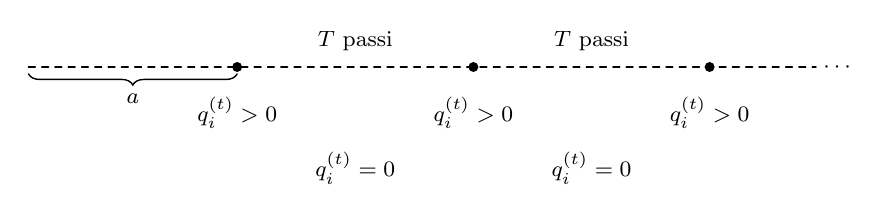
\begin{tikzpicture}[x=1cm,y=1cm,font=\footnotesize,line cap=round,
    asse/.style={line width=0.6pt,dash pattern=on 2.4pt off 2.4pt},
    pallino/.style={circle,fill=black,inner sep=0pt,minimum size=3.6pt}]

  % ------------------------------------------------------- asse dei tempi ---
  \draw[asse] (0.15,0) -- (10.15,0);
  \node[anchor=west,inner sep=2.5pt] at (10.15,0) {$\cdots$};

  % --------------------------------------- gli istanti a, a+T, a+2T, ... ----
  \node[pallino] at (2.80,0) {};
  \node[pallino] at (5.80,0) {};
  \node[pallino] at (8.80,0) {};

  % ------------------------------------ graffa dello sfasamento iniziale ----
  \draw[line width=0.5pt,decorate,
        decoration={brace,mirror,amplitude=4pt,raise=2.5pt}]
       (0.15,0) -- (2.80,0);
  \node[anchor=north,inner sep=1.5pt] at (1.475,-0.28) {$a$};

  % ----------------------------- etichette degli istanti «buoni» (pallini) --
  \node[anchor=north,inner sep=1.5pt] at (2.80,-0.32) {$q_i^{(t)}>0$};
  \node[anchor=north,inner sep=1.5pt] at (5.80,-0.32) {$q_i^{(t)}>0$};
  \node[anchor=north,inner sep=1.5pt] at (8.80,-0.32) {$q_i^{(t)}>0$};

  % -------------------------------- etichette degli intervalli fra pallini --
  \node[anchor=south,inner sep=1.5pt] at (4.30,0.14) {$T$ passi};
  \node[anchor=south,inner sep=1.5pt] at (7.30,0.14) {$T$ passi};

  \node[anchor=north,inner sep=1.5pt] at (4.30,-1.02) {$q_i^{(t)}=0$};
  \node[anchor=north,inner sep=1.5pt] at (7.30,-1.02) {$q_i^{(t)}=0$};

\end{tikzpicture}

  \caption{La periodicità letta sull'asse dei tempi: lo stato $i$ può essere occupato
  ($q_i^{(t)}>0$) soltanto negli istanti $a,\,a+T,\,a+2T,\dots$, mentre in tutti gli altri
  istanti si ha $q_i^{(t)}=0$.}
  \label{fig:p78-periodicita}
\end{figure}

\begin{osservazione}
  Prendendo $\vec{q}^{\,(0)}$ concentrata in $i$ si ha $q_i^{(0)} = 1 > 0$, il che forza
  $a \equiv 0$, e la condizione diventa: $T$ divide ogni $t$ per cui $P_{ii}^{(t)}>0$. Con
  questa scelta la periodicità di $i$ è il massimo comune divisore dell'insieme
  $\set{t\ge 1 \;:\; P_{ii}^{(t)}>0}$ dei possibili tempi di ritorno in $i$, e il massimo
  esiste davvero non appena in $i$ si può tornare: $T=1$ è sempre ammissibile, e ogni $T$
  ammissibile divide --- dunque non supera --- un qualunque tempo di ritorno. La
  quantificazione esistenziale su $\vec{q}^{\,(0)}$ non cambia il valore per le catene
  irriducibili, che sono poi le sole per cui useremo la nozione; in generale, invece, la
  renderebbe inservibile, perché una distribuzione iniziale da cui $i$ non è raggiungibile
  soddisfa la condizione a vuoto, per ogni $T$.
\end{osservazione}

\begin{definizione}[Stati e catene aperiodiche]\label{def:mc-aperiodica}
  Lo stato $i$ è \emph{periodico} se ha periodicità $>1$; altrimenti è \emph{aperiodico}.
  Una catena è \emph{aperiodica} se ogni suo stato lo è.
\end{definizione}

\begin{definizione}[Stati e catene ergodiche]\label{def:mc-ergodico}
  Uno stato è \emph{ergodico} se è
  \begin{itemize}
    \item aperiodico;
    \item persistente non nullo.
  \end{itemize}
  Una catena di Markov è \emph{ergodica} se ogni suo stato lo è.
\end{definizione}

\begin{osservazione}
  I due requisiti, messi insieme, dicono che un random walk sulla catena ritorna in quello
  stato con probabilità $1$ (persistenza), dopo un tempo di attesa di valore atteso finito
  (non nullità) e senza che gli istanti di visita siano confinati in una progressione
  aritmetica (aperiodicità): il random walk continua dunque a visitare, indefinitamente nel
  tempo, ogni suo stato.
\end{osservazione}

\begin{teorema}[fondamentale sulle catene di Markov]\label{thm:mc-fondamentale}
  Ogni catena di Markov irriducibile, finita e aperiodica gode delle seguenti proprietà.
  \begin{enumerate}
    \item Tutti i suoi stati sono ergodici.
    \item Esiste una distribuzione stazionaria $\vec{\pi}$ tale che $\pi_i>0$ per ogni $i$.
    \item Per ogni $i$ si ha
      \[
        f_{ii}=1 \qquad\text{e}\qquad h_{ii}=\frac{1}{\pi_i}.
      \]
    \item \scan{79}%
      Detto $N(i,t)$ il numero medio di volte in cui la catena visita lo stato $i$ nei
      primi $t$ passi, vale
      \[
        \lim_{t\to\infty}\frac{N(i,t)}{t}=\pi_i .
      \]
  \end{enumerate}
\end{teorema}

\begin{osservazione}
  La distribuzione stazionaria del punto~2 è anche \emph{unica}, e i punti~3 e~4 ne danno
  due letture concrete. Il punto~3 dice che $\pi_i$ è il reciproco del tempo medio di
  ritorno in $i$; il punto~4 è la lettura «frequentista»: $\pi_i$ è la frazione di tempo
  che la catena trascorre, alla lunga, nello stato $i$. Le due letture sono coerenti fra
  loro: se il tempo medio di ritorno in $i$ è $h_{ii}=1/\pi_i$, in $t$ passi lo stato $i$
  viene visitato circa $t\,\pi_i$ volte.

  Sotto le stesse ipotesi vale inoltre il \emph{basic limit theorem}: qualunque sia la
  distribuzione iniziale $\vec{q}^{\,(0)}$ si ha $\vec{q}^{\,(t)} \to \vec{\pi}$ per
  $t\to\infty$. È il fatto usato nell'Esempio~\ref{es:ciclo6}, e va tenuto distinto dal
  punto~4: quello è un limite alla Cesàro e continua a valere per le catene irriducibili
  \emph{periodiche}, per le quali invece $\vec{q}^{\,(t)}$ in generale non converge.
\end{osservazione}
